\documentclass[a4paper]{article}
\usepackage{ctex}
\usepackage{amsmath, amssymb, amsthm}
\usepackage{array}
\usepackage{moreenum}
\usepackage{mathtools}
\usepackage{url}
\usepackage{bm}
\usepackage{enumitem}
\usepackage{graphicx}
\usepackage{listings}
\usepackage{xcolor}
\usepackage{multirow}
\usepackage{diagbox}
\usepackage{float}
\usepackage[top=1.5cm, bottom=1.5cm, left=1.5cm, right=1.5cm]{geometry}
\lstset{
    basicstyle          =   \sffamily,          % 基本代码风格
    keywordstyle        =   \bfseries,          % 关键字风格
    commentstyle        =   \rmfamily\itshape,  % 注释的风格，斜体
    stringstyle         =   \ttfamily,  % 字符串风格
    flexiblecolumns,                % 
    numbers             =   left,   % 行号的位置在左边
    showspaces          =   false,  % 是否显示空格，显示了有点乱，所以不现实了
    numberstyle         =   \zihao{-5}\ttfamily,    % 行号的样式，小五号，tt等宽字体
    showstringspaces    =   false,
    captionpos          =   t,      % 这段代码的名字所呈现的位置，t指的是top上面
    frame               =   lrtb,   % 显示边框
}

\lstdefinestyle{Python}{
    language        =   Python, % 语言选Python
    basicstyle      =   \zihao{-5}\ttfamily,
    numberstyle     =   \zihao{-5}\ttfamily,
    keywordstyle    =   \color{blue},
    keywordstyle    =   [2] \color{teal},
    stringstyle     =   \color{magenta},
    commentstyle    =   \color{red}\ttfamily,
    breaklines      =   true,   % 自动换行，建议不要写太长的行
    columns         =   fixed,  % 如果不加这一句，字间距就不固定，很丑，必须加
    basewidth       =   0.5em,
}
% \usepackage{subcaption}
\usepackage[caption=false,font=footnotesize,labelfont=rm,textfont=rm,subrefformat=parens]{subfig}
\usepackage{booktabs} % toprule
\usepackage[mathcal]{eucal}
\usepackage{color}
\usepackage{iidef}
\newif\ifans\anstrue
\newcommand{\myspace}[1]{\par\vspace{#1\baselineskip}}

\thecourseinstitute{\textnormal{媒体与认知}}
\theterm{确定}
\begin{document}



\vspace{3mm}
\centerline{\textbf{\Large{媒体与认知课程上机作业中期报告：基于SigLIP的小规模图文检索系统}}}
\centerline{\textbf{{徐一 $\quad$ 2023010514 $\quad$ 无32}}}


\section{项目背景}

多模态学习（Multimodal Learning）是当前人工智能领域的研究热点，其中视觉与语言的融合任务，如图文匹配、图文检索、图文生成等，具有广泛的应用前景。

CLIP（Contrastive Language–Image Pretraining）是 OpenAI 提出的多模态预训练方法，利用图像-文本对比学习，使模型能自动将图像和文本嵌入到同一语义空间中，进而支持多种下游任务。然而该方案存在诸多问题，如强依赖大 batch size。

SigLIP（Sigmoid Loss for Language-Image Pretraining）是由 Google Research 提出的一种视觉-语言预训练方法，是对经典对比学习框架（如 CLIP）的重要改进。

\section{任务目标}

1. 理解 CLIP 与 SigLIP 在损失函数上的差异。

2. 使用Pytorch实现图像编码器、文本编码器和 SigLIP 损失函数。

3. 在 Flickr8k 数据集上训练模型，并报告 Text-to-Image 与 Image-to-Text 的 Recall@1/5/10。

4. 分析模型在多模态语义对齐方面的效果及可视化结果。

5. 基于 google/siglip-base-patch16-224 预训练模型，体验图文跨模态对比学习的核心结果——图文交叉相似度矩阵。


\section{技术路线与方法}

\subsection{数据及选择}

使用 Flickr8k 数据集，数据格式为图像 + 文字描述（1-5 条）。

\subsection{模型结构}

\begin{figure}[H]
    \centering
    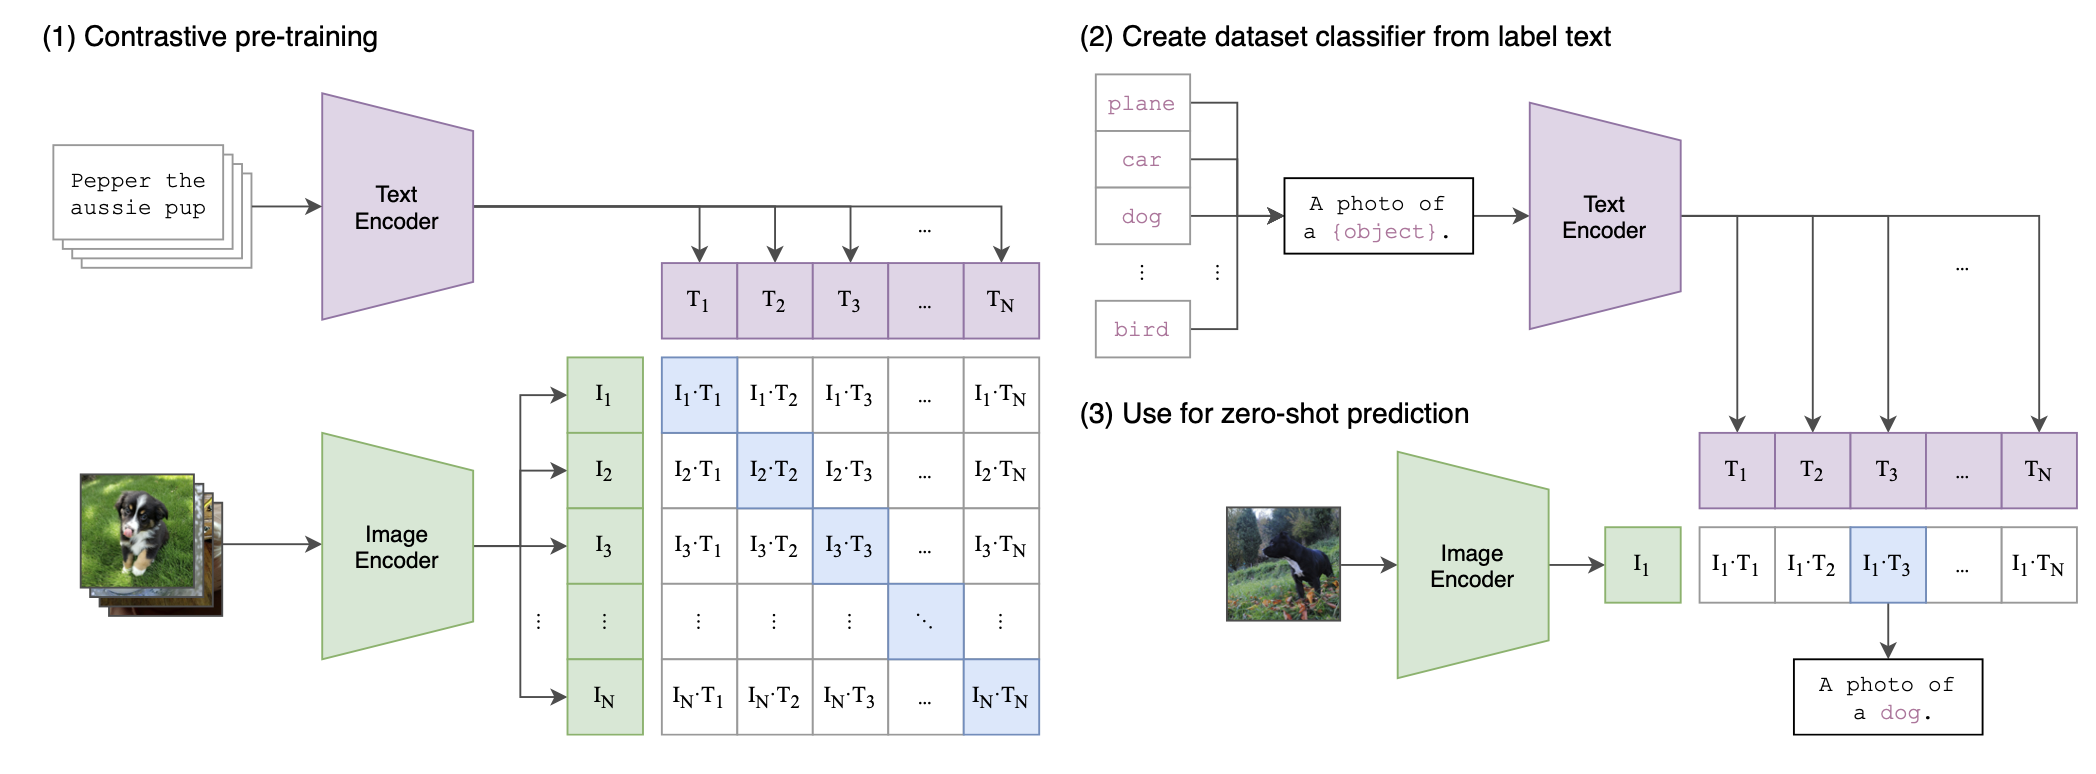
\includegraphics[width=0.8\textwidth]{model_arch.png}
    \caption{模型结构}
    \label{fig:model}
\end{figure}

\begin{itemize}
    \item \textbf{图像编码器【Task1】}
    \begin{itemize}
        \item 使用 ResNet18 进行特征提取，输出特征向量。
        \item 添加线性层映射到共享语义空间。
    \end{itemize}
    
    \item \textbf{文本编码器【Task2】}
    \begin{itemize}
        \item 使用 MLP 或 Transformer 提取文本表示。
        \item 线性层将文本特征映射到相同维度的共享空间。
    \end{itemize}
    
    \item \textbf{SigLIP损失函数【Task3】}
    \begin{itemize}
        \item SigLIP Loss（Sigmoid-based）
        
        设图像编码为 $z_i^{I}$，文本编码为 $z_j^{T}$，相似度仍采用余弦相似度。
        
        设一个 batch 中包含 $|\mathcal{B}|$ 个图文样本对，图像编码为 $x_i$，文本编码为 $y_j$，二者的相似度定义为：
        \[
        z_{ij} = \frac{x_i^\top y_j}{\|x_i\| \, \|y_j\|}
        \]
        其中，$t$ 为可学习的温度系数，$b$ 为可学习的偏置项。定义图文匹配标签为：
        \[
        s_{ij} =
        \begin{cases}
        +1, & i = j \\
        -1, & i \ne j
        \end{cases}
        \]
        则对于任意一对 $(i,j)$，SigLIP 的成对损失为：
        \[
        \mathcal{L}_{ij} = \log \left( 1 + \exp\left( s_{ij} \, (-t z_{ij} + b) \right) \right)
        \]
        因此，整个 batch 上的 SigLIP 损失为：
        \[
        \mathcal{L}_{\text{SigLIP}}
        =
        \frac{1}{|\mathcal{B}|}
        \sum_{i=1}^{|\mathcal{B}|}
        \sum_{j=1}^{|\mathcal{B}|}
        \mathcal{L}_{ij}
        \]
        即
        \[
        \mathcal{L}_{\text{SigLIP}}
        =
        \frac{1}{|\mathcal{B}|}
        \sum_{i=1}^{|\mathcal{B}|}
        \sum_{j=1}^{|\mathcal{B}|}
        \log \left( 1 + \exp\left( s_{ij} \, (-t z_{ij} + b) \right) \right)
        \]
    \end{itemize}
\end{itemize}


\section{训练流程}

    1. 图像 + 文本 输入模型 

    2. 提取图像特征 / 文本特征

    3. 归一化后计算余弦相似度矩阵
    
    4. 计算损失并反向传播

    5. 每轮评估 Top-K Accuracy / Recall@K 检索准确率，保存最优模型

\section{实验环境}

1. GPU型号：NVIDIA GeForce RTX 5090

2. PyTorch版本：2.11.0


\section{结果分析与可视化}

\subsection{Sanity Check}

运行命令

\begin{lstlisting}
$ python train_siglip.py --dry-run --epochs 2 --batch-size 32 --num-workers 0
\end{lstlisting}

发现训练可以正常运行，运行结果保存至\texttt{outputs/siglip\_resnet\_transformer/}目录下。


\subsection{训练 Resnet + Transformer}

运行命令

\begin{lstlisting}
$ python train_siglip.py \
$  --data-dir Flickr8k \
$  --text-encoder transformer \
$  --epochs 20 \
$  --batch-size 64 \
$  --output-dir outputs/resnet_transformer
\end{lstlisting}

lr为默认值$1\times 10^{-4}$。训练loss曲线和最终测试集输出结果如下，运行结果保存至\texttt{outputs/resnet\_transformer/}目录下。

\begin{figure}[H]
    \centering
    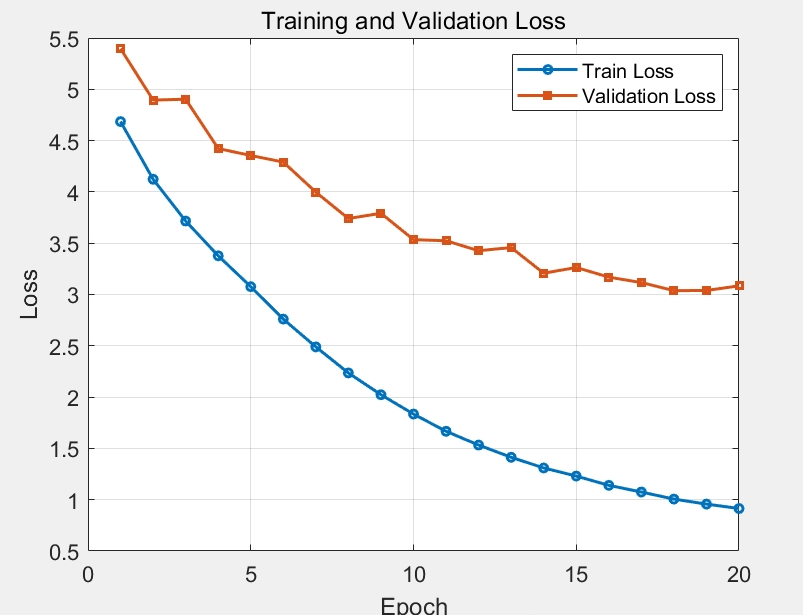
\includegraphics[width=0.6\textwidth]{loss2.png}
    \caption{ResNet + Transformer 模型训练loss曲线}
    \label{fig:Tloss}
\end{figure}

$final \quad test\_loss=3.0497$。训练效果较好。

\begin{table}[H]
    \centering
    \begin{tabular}{c|ccc|ccc}
        \hline
        \multirow{2}{*}{Model} & \multicolumn{3}{c|}{Text-to-Image} & \multicolumn{3}{c}{Image-to-Text} \\
        & R@1 & R@5 & R@10 & R@1 & R@5 & R@10 \\
        \hline
        ResNet + Transformer & 11.84 & 30.65 & 42.88 & 12.04 & 31.61 & 42.83 \\
        \hline
    \end{tabular}
    \caption{ResNet + Transformer 模型在 Flickr8k 上的检索结果}
    \label{tab:results}
\end{table}


\subsection{轻量文本baseline}

运行命令

\begin{lstlisting}
$ python train_siglip.py \
$   --data-dir Flickr8k \
$   --text-encoder mlp \
$   --epochs 20 \
$   --batch-size 64 \
$   --output-dir outputs/resnet_mlp
\end{lstlisting}

lr为默认值$1\times 10^{-4}$。训练loss曲线和最终测试集输出结果如下，运行结果保存至\texttt{outputs/resnet\_mlp}目录下。

\begin{figure}[H]
    \centering
    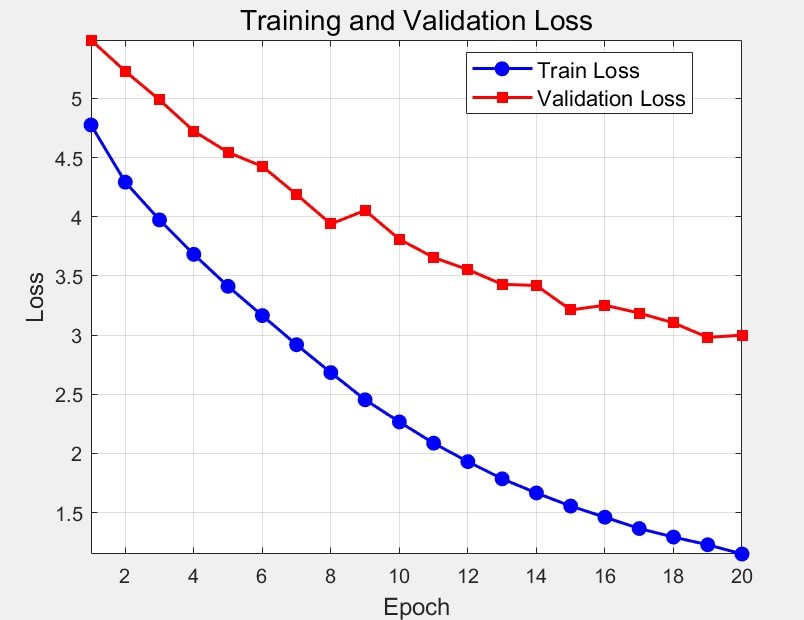
\includegraphics[width=0.6\textwidth]{loss1.png}
    \caption{ResNet + MLP 模型训练loss曲线}
    \label{fig:MLPloss}
\end{figure}

$final \quad test\_loss=3.0192$。训练效果较好。

\begin{table}[H]
    \centering
    \begin{tabular}{c|ccc|ccc}
        \hline
        \multirow{2}{*}{Model} & \multicolumn{3}{c|}{Text-to-Image} & \multicolumn{3}{c}{Image-to-Text} \\
        & R@1 & R@5 & R@10 & R@1 & R@5 & R@10 \\
        \hline
        ResNet + MLP & 11.15 & 31.07 & 42.91 & 11.37 & 30.91 & 42.74 \\
        \hline
    \end{tabular}
    \caption{ResNet + MLP 模型在 Flickr8k 上的检索结果}
    \label{tab:results_mlp}
\end{table}


可见，两者性能接近，在 Text-to-Image 检索上轻量文本baseline甚至略优于 ResNet + Transformer 模型。


分析原因可能为:

\quad \quad 1. 图像编码器 ResNet18 参数过少、性能较差，影响了模型的性能上限；

\quad \quad 2. 文本编码器采用平均池化，将所有 token 同等对待，使得模型退化，没有通过注意力机制学习到的顺序和交互信息；

\quad \quad 3. Flickr8k 数据规模小，Transformer 学习不充分；

\quad \quad 4. 学习率、温度、batch size等参数未进行充分调优，可能影响了模型的性能表现。

\quad \quad 5. 预训练初始化的权重可能不适合当前任务，导致模型在小规模数据集上表现不佳。


笔者认为可能的优化方向有：

\quad \quad 1. 微调训练超参数，增大epoch数；

\quad \quad 2. 增强图像编码器，如增大 --image-width；

\quad \quad 3. Transformer 引入其他更合适的池化方式。

\quad \quad 4. 优化与训练初始化的策略。

\quad \quad 5. 数据增强。


\subsection{可视化}

编写文本 $\rightarrow$ 图像 Top-K 检索示例的可视化代码，见 \texttt{visualize\_topk.py}。

运行命令

\begin{lstlisting}
$ python visualize_topk.py \
$   --data-dir Flickr8k \
$   --checkpoint outputs/resnet_transformer/best_siglip.pt \
$   --split test \
$   --topk 5 \
$   --num-queries 8 \
$   --output-dir outputs/topk_vis_transformer
\end{lstlisting}

得到 Top-5 检索结果，取几次检索结果如下图所示，图像保存在 \texttt{/outputs/topk\_vis\_transformer/} 下。

\begin{figure}[H]
    \centering
    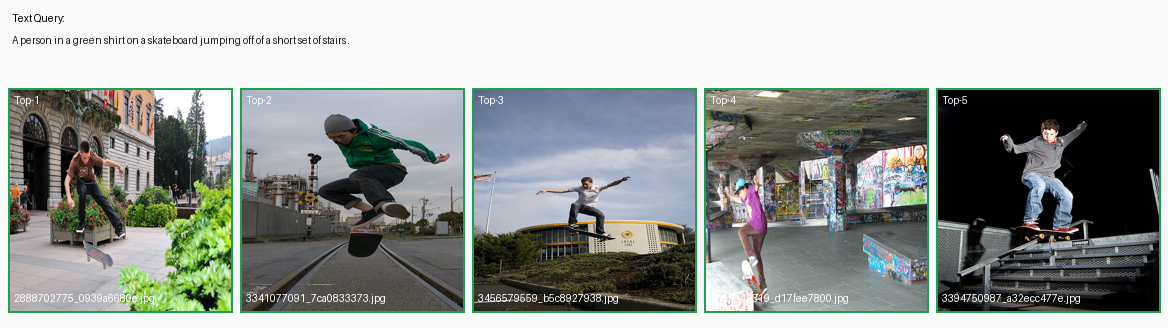
\includegraphics[width=0.8\textwidth]{query_05.png}
    \caption{文本 $\rightarrow$ 图像 Top-5 检索结果示例1}
    \label{fig:visualization}
\end{figure}

\begin{figure}[H]
    \centering
    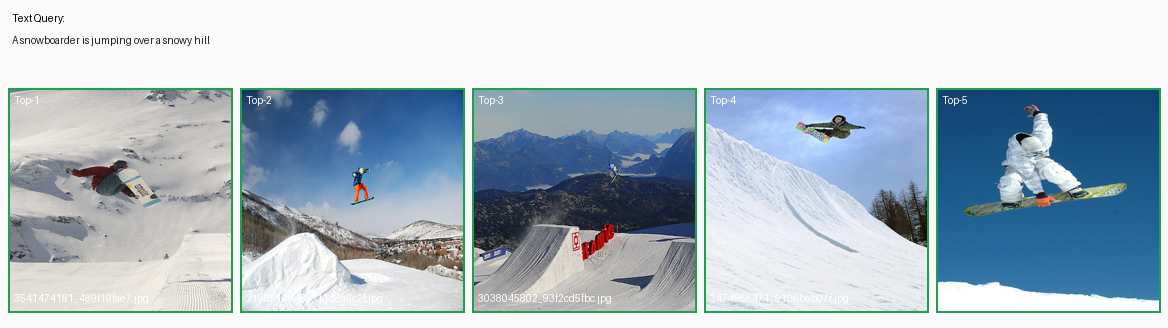
\includegraphics[width=0.8\textwidth]{query_04.png}
    \caption{文本 $\rightarrow$ 图像 Top-5 检索结果示例2}
    \label{fig:visualization}
\end{figure}

\begin{figure}[H]
    \centering
    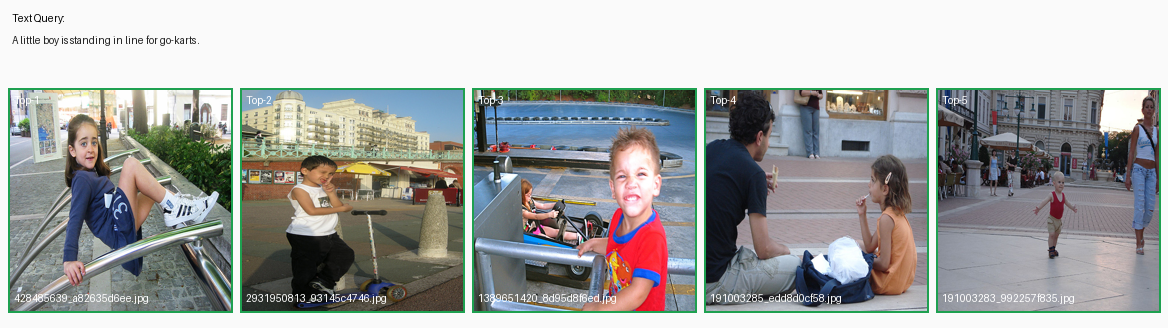
\includegraphics[width=0.8\textwidth]{query_03.png}
    \caption{文本 $\rightarrow$ 图像 Top-5 检索结果示例3}
    \label{fig:visualization}
\end{figure}

\begin{figure}[H]
    \centering
    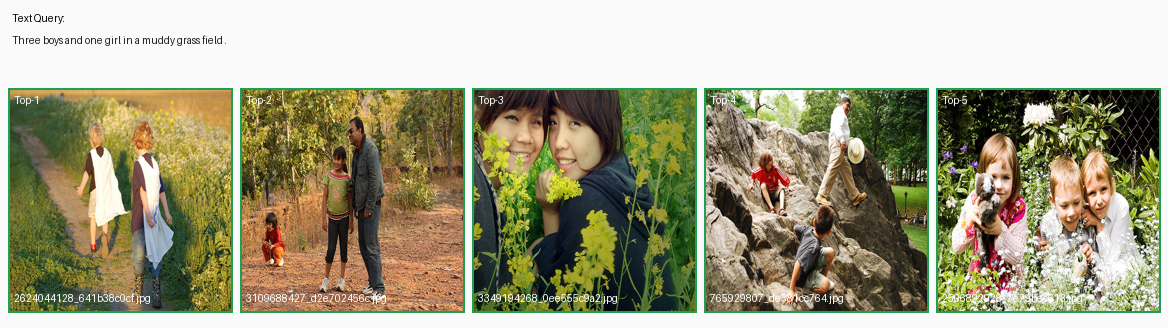
\includegraphics[width=0.8\textwidth]{query_06.png}
    \caption{文本 $\rightarrow$ 图像 Top-5 检索结果示例4}
    \label{fig:visualization}
\end{figure}


对比以上四次检索结果，可以发现前两个示例的检索较准确，而后两个较差。具体来说，基于当前的训练情况，模型在一些简单的场景（如单人、物体较少）上表现较好，但在复杂场景（如多人、多物体）尤其是对男女性别判断上存在较大问题。


\section{图文交叉相似度矩阵}

在\texttt{visualization/}目录下运行命令

\begin{lstlisting}
$ pip install -r requirements.txt
$ export HF_ENDPOINT=https://hf-mirror.com
$ python app.py
\end{lstlisting}

访问 \texttt{http://localhost:7860}，取图文对数量为8，随机采样并生成热力图如下所示：

\begin{figure}[H]
    \centering
    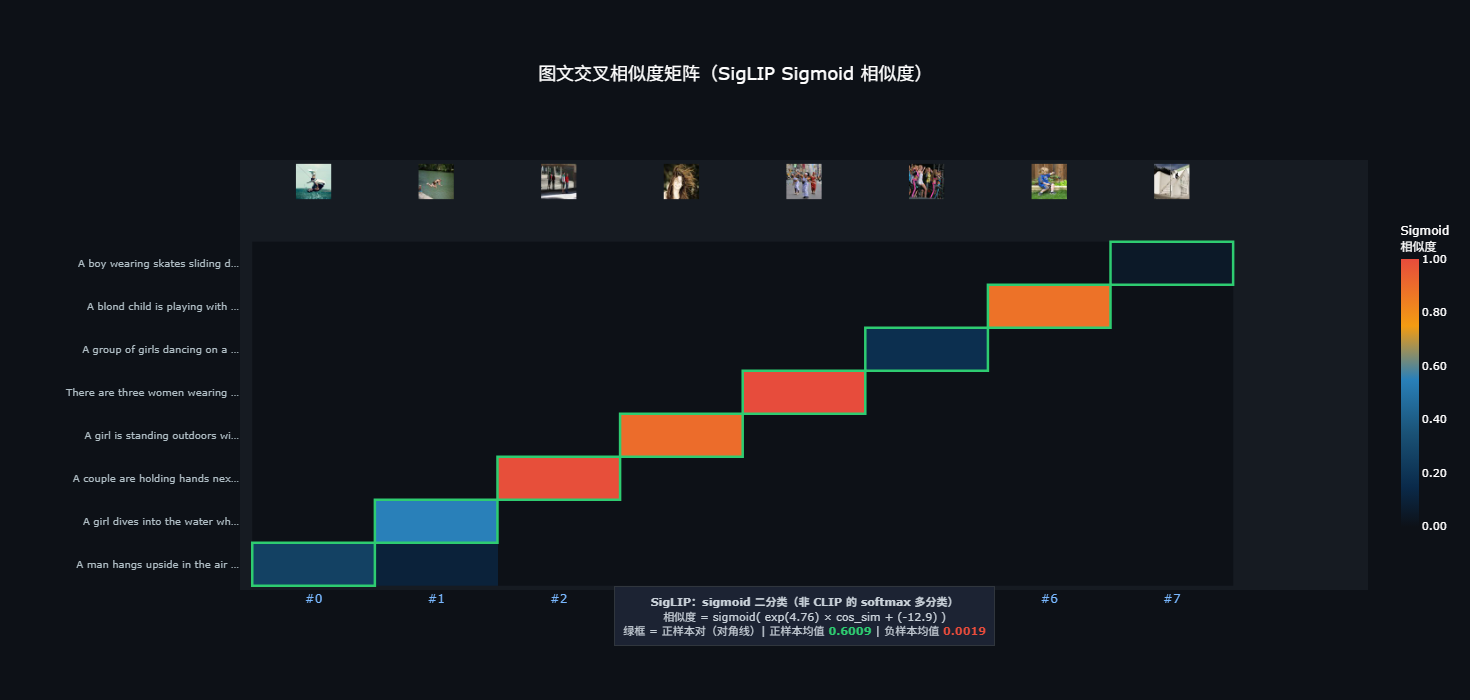
\includegraphics[width=0.8\textwidth]{newplot.png}
    \caption{图文交叉相似度矩阵可视化示例}
    \label{fig:cross_modal_similarity}
\end{figure}

数据分析：

\begin{figure}[H]
    \centering
    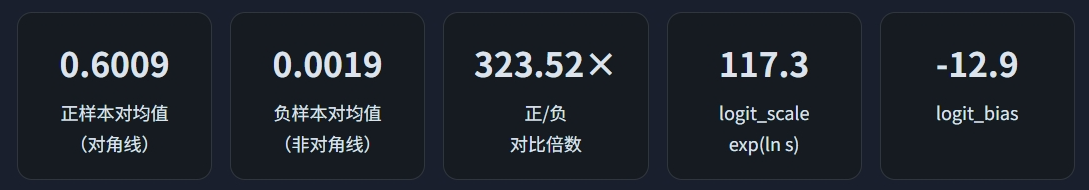
\includegraphics[width=0.8\textwidth]{image.png}
    \caption{图文交叉相似度矩阵数据分析}
    \label{fig:cross_modal_similarity}
\end{figure}


\section{优化实验}

前文baseline实验采用 20 个 epoch 训练，从 loss 曲线可见损失尚未充分收敛，因此不宜作为优化对比的参照。本节统一将训练轮数固定为 40 epoch，以 ResNet + Transformer、lr=$3\times 10^{-4}$、\texttt{image\_width=32}、平均池化为baseline，在此基础上分别加入各单项优化进行消融实验。所有实验 batch size 均为 64，评估指标与baseline训练一致。

\subsection{优化实现}

    1. 超参数优化，在 40 epoch 基础上，将学习率设为 $1\times 10^{-4}$，并加入 3 轮 warmup 与 cosine 学习率衰减（\texttt{--use-cosine-lr}）。

    2. 增强图像编码器，将 ResNet 基础通道宽度由 32 增大至 48（\texttt{--image-width 48}）。

    3. 改进池化方式，在 Transformer 文本编码器中采用可学习 [CLS] token 池化（\texttt{--pool-type cls}）或 max 池化（\texttt{--pool-type max}），与baseline的平均池化对比。

    4. 初始化策略，对 Linear 使用 Xavier、对 Conv 使用 Kaiming、对 Embedding 使用小方差正态分布（\texttt{--custom-init}）。

    5. 数据增强，在训练集上对图像施加随机水平翻转（\texttt{RandomHorizontalFlip}，$p=0.5$）与颜色抖动（\texttt{ColorJitter}），通过 \texttt{--data-aug} 开关启用；验证集与测试集不做增强。

\subsection{消融实验}

baseline命令如下，运行结果保存至 \texttt{outputs/baseline\_transformer/} 目录：

\begin{lstlisting}
$ python train_siglip.py \
$   --data-dir Flickr8k \
$   --text-encoder transformer \
$   --epochs 40 \
$   --batch-size 64 \
$   --lr 3e-4 \
$   --image-width 32 \
$   --pool-type mean \
$   --output-dir outputs/baseline_transformer
\end{lstlisting}

在baseline配置基础上，分别单独启用各优化项，命令如下：


\textbf{仅超参数}
\begin{lstlisting}
$ python train_siglip.py --data-dir Flickr8k --text-encoder transformer \
$   --epochs 40 --batch-size 64 --lr 1e-4 --warmup-epochs 3 --use-cosine-lr \
$   --output-dir outputs/ablate_hparams
\end{lstlisting}

\textbf{仅加宽 ResNet}

\begin{lstlisting}
$ python train_siglip.py --data-dir Flickr8k --text-encoder transformer \
$   --epochs 40 --batch-size 64 --image-width 48 \
$   --output-dir outputs/ablate_image_width
\end{lstlisting}

\textbf{仅 CLS 池化 / Max 池化 / 自定义初始化}

\begin{lstlisting}
$ python train_siglip.py ... --pool-type cls --output-dir outputs/ablate_pool_cls
$ python train_siglip.py ... --pool-type max --output-dir outputs/ablate_pool_max
$ python train_siglip.py ... --custom-init --output-dir outputs/ablate_init
\end{lstlisting}

\textbf{仅数据增强}

\begin{lstlisting}
$ python train_siglip.py --data-dir Flickr8k --text-encoder transformer \
$   --epochs 40 --batch-size 64 --lr 3e-4 --data-aug \
$   --output-dir outputs/ablate_data_aug
\end{lstlisting}

测试集结果汇总如下（指标取自各目录下 \texttt{train.log} 末尾）：

\begin{table}[H]
    \centering
    \begin{tabular}{c|c|ccc|ccc}
        \hline
        \multirow{2}{*}{实验配置} & \multirow{2}{*}{test\_loss} & \multicolumn{3}{c|}{Text-to-Image} & \multicolumn{3}{c}{Image-to-Text} \\
        & & R@1 & R@5 & R@10 & R@1 & R@5 & R@10 \\
        \hline
        baseline（40 epoch，无额外优化） & 3.1387 & 16.83 & 38.28 & 49.53 & 18.57 & 38.84 & 50.49 \\
        仅超参数（cosine lr） & 2.0826 & 26.17 & 51.68 & 62.88 & 28.91 & 53.59 & 64.80 \\
        仅加宽 ResNet（width=48） & 3.0503 & 18.04 & 39.97 & 51.80 & 18.78 & 41.06 & 52.83 \\
        仅 CLS 池化 & 2.9386 & 15.50 & 37.91 & 49.75 & 17.51 & 39.06 & 51.49 \\
        仅 Max 池化 & 2.9107 & 18.54 & 41.57 & 51.98 & 20.15 & 41.79 & 52.64 \\
        仅自定义初始化 & 3.0332 & 11.64 & 32.01 & 44.91 & 12.13 & 33.98 & 46.47 \\
        仅数据增强（flip + color jitter） & 3.2909 & 16.39 & 36.06 & 47.38 & 16.08 & 37.75 & 48.69 \\
        \hline
    \end{tabular}
    \caption{40 epoch baseline与各优化方向的消融实验测试集结果}
    \label{tab:ablation}
\end{table}

$\text{final test\_loss}=3.1387$（baseline）。与 20 epoch baseline相比，40 epoch baseline的 Text-to-Image R@1 由 12.38\% 提升至 16.83\%，说明延长训练确实有助于模型收敛。在此基础上，单项优化有提升的是超参数、加宽 Resnet 和 Max 池化。

\subsection{优化效果分析}

根据 40 epoch 下的消融实验，可以得到以下结论：

1. 固定 40 epoch 后，baseline性能明显高于 20 epoch 设置。 baseline t2i\_R@1 从 12.38\% 升至 16.83\%，验证了“20 epoch 时损失未收敛”的判断。

2. 超参数调整（cosine lr + $1\times 10^{-4}$）是本次最有效的单项优化。 在 40 epoch baseline上，t2i\_R@1 由 16.83\% 提升至 26.17\%，i2t\_R@1 由 18.57\% 提升至 28.91\%，测试损失由 3.14 降至 2.08。

3. 加宽 ResNet 有小幅提升。 将 \texttt{image\_width} 增至 48 后，t2i\_R@1 为 18.04\%，略高于baseline（16.83\%），但 test\_loss 与baseline接近（3.05 vs.\ 3.14）。更宽的视觉编码器在小规模数据上有一定帮助，但提升有限，可能受限于数据规模与训练轮数。

4. Max 池化略优于平均池化，CLS 池化反而更差。 Max 池化使 t2i\_R@1 升至 18.54\%，i2t\_R@1 升至 20.15\%，略优于baseline；CLS 池化则降至 15.50\% / 17.51\%。

5. 自定义初始化损害性能。 启用 custom init 后，t2i\_R@1 降至 11.64\%，低于 20 epoch baseline水平。 可能是预训练权重更适合当前任务，自定义初始化导致模型难以收敛。

6. 数据增强没有帮助。 启用数据增强后，t2i\_R@1 由 16.83\% 降至 16.39\%，i2t\_R@1 由 18.57\% 降至 16.08\%，测试损失由 3.14 升至 3.29，说明在当前任务与数据规模下，随机翻转与颜色抖动可能引入了过多噪声，反而损害了模型的对齐能力。


\subsection{综合优化策略与最终结果}

综合前述消融实验，经过多次实验测试，本文最终选取以下三项有效优化进行组合：\textbf{超参数调整}（lr=$1\times 10^{-4}$、warmup 3 epoch、cosine 学习率衰减）、\textbf{加宽 ResNet}（\texttt{image\_width=48}）与 \textbf{Max 池化}（\texttt{--pool-type max}）。未采用 CLS 池化、自定义初始化与数据增强。

关于训练轮数：40 epoch baseline在 epoch 38--40 附近验证集 Recall 趋于饱和（t2i\_R@1 约 14.8\%--16.5\%），继续训练损失有反弹迹象，baseline对比统一取 40 epoch。综合优化后模型参数量更大、学习率更低，收敛更慢，在 40 epoch 时验证集 t2i\_R@1 约为 31.3\%，至 64 epoch 仍可继续提升至约 33.6\%，最终方案采用 64 epoch。

运行命令如下，结果保存至 \texttt{outputs/optim\_hparams\_imagewidth\_maxpool\_more/} 目录：

\begin{lstlisting}
$ python train_siglip.py \
$   --data-dir Flickr8k \
$   --text-encoder transformer \
$   --epochs 64 \
$   --batch-size 64 \
$   --lr 1e-4 \
$   --warmup-epochs 3 \
$   --use-cosine-lr \
$   --image-width 48 \
$   --pool-type max \
$   --output-dir outputs/optim_hparams_imagewidth_maxpool_more
\end{lstlisting}

训练loss曲线和最终测试集输出结果如下：

\begin{figure}[H]
    \centering
    \includegraphics[width=0.6\textwidth]{image copy.png}
    \caption{综合优化训练loss曲线}
    \label{fig:allloss}
\end{figure}

测试集最终结果与 40 epoch baseline对比如下：

\begin{table}[H]
    \centering
    \begin{tabular}{c|c|ccc|ccc}
        \hline
        \multirow{2}{*}{Model} & \multirow{2}{*}{test\_loss} & \multicolumn{3}{c|}{Text-to-Image} & \multicolumn{3}{c}{Image-to-Text} \\
        & & R@1 & R@5 & R@10 & R@1 & R@5 & R@10 \\
        \hline
        baseline（40 epoch） & 3.1387 & 16.83 & 38.28 & 49.53 & 18.57 & 38.84 & 50.49 \\
        综合优化（64 epoch） & 2.2124 & 36.73 & 59.91 & 68.88 & 37.90 & 61.28 & 70.24 \\
        \hline
    \end{tabular}
    \caption{40 epoch baseline与综合优化模型在 Flickr8k 测试集上的检索结果对比}
    \label{tab:final_optimized}
\end{table}

$\text{final test\_loss}=2.2124$。与 40 epoch baseline相比，综合优化在 Text-to-Image 的 R@1 上提升约 19.9 个百分点（16.83\% $\rightarrow$ 36.73\%），R@5 提升约 21.6 个百分点，R@10 提升约 19.4 个百分点；Image-to-Text 的 R@1 提升约 19.3 个百分点（18.57\% $\rightarrow$ 37.90\%），R@5 提升约 22.4 个百分点，R@10 提升约 19.8 个百分点；测试损失由 3.14 降至 2.21。

最终分析：

1. 最终最有效的优化方案为超参数（cosine lr） + Max 池化 + 加宽 Resnet。单独超参数优化在 40 epoch 下 t2i\_R@1 为 26.17\%；单独加宽 ResNet 为 18.04\%；单独 Max 池化为 18.54\%。组合后在 64 epoch 下达到 36.73\%，说明更宽的视觉编码器、更合适的池化方式与 cosine 学习率策略能相互促进，但需要更长训练充分收敛。

2. Max 池化优于 CLS 池化。 消融实验中 Max 池化在 40 epoch baseline上略优于 mean 与 cls，最终方案选用 max pooling，和 Transformer 文本侧保留 token 特征的需求一致。

3. epoch 数需与模型复杂度匹配。 baseline模型较简单，40 epoch 已接近最优；综合优化后模型容量与学习率 schedule 均改变，64 epoch 时验证集 Recall 仍高于 40 epoch（t2i\_R@1 由 31.3\% 升至 33.6\%），说明对优化配置来说 40 epoch 训练不够，而非过拟合。

4. 与预训练 SigLIP 仍有差距，但自训练模型有很大提升。 综合优化后 Recall 接近 37\%，较初始 20 epoch baseline（t2i\_R@1 约 12\%）提升很大，距离预训练大模型仍有差距，主要受限于 Flickr8k 数据规模与模型容量。


\end{document}